\documentclass[aspectratio=1610]{beamer}
\usepackage[utf8]{inputenc}
\usepackage{sansmathfonts}
\usepackage[T1]{fontenc}

\usepackage[natbib=true,style=numeric,sorting=none]{biblatex}
\addbibresource{references.bib}

\usepackage{caption}
\usepackage{subcaption}
\usepackage{algorithm}
\usepackage{algpseudocode}
\usepackage{amsmath,amssymb,amsfonts}

\usepackage{tikz}
\usetikzlibrary{arrows.meta}
\usetikzlibrary{tikzmark}
\usetikzlibrary{backgrounds,calc,positioning}
\usetikzlibrary{shapes,decorations.pathreplacing}

\usepackage{listings}

\usetheme{main}

\captionsetup{font=scriptsize,labelfont=scriptsize}

\title[CM2 - Représentation d'informations]{CM2 - Représentation d'informations dans un ordinateur}

\date[]{}
\author[AM]{\textbf{Ammar Mian} \\ \footnotesize Associate professor, LISTIC, Université Savoie Mont Blanc \\ POLYTECH Annecy-Chambéry}

\newcommand{\red}[1]{\textcolor{red}{#1}}

%%%%% BASIC MATH DEFINITIONS %%%%%

\usepackage{amsmath,amsfonts,bm}

% Figure references
\def\figref#1{figure~\ref{#1}}
\def\Figref#1{Figure~\ref{#1}}

% Section references
\def\secref#1{section~\ref{#1}}
\def\Secref#1{Section~\ref{#1}}

% Algorithm references
\def\algref#1{algorithm~\ref{#1}}
\def\Algref#1{Algorithm~\ref{#1}}

% Common mathematical sets
\def\R{{\mathbb{R}}}
\def\N{{\mathbb{N}}}
\def\Z{{\mathbb{Z}}}
\def\C{{\mathbb{C}}}

% Common operations
\DeclareMathOperator{\Tr}{Tr}
\newcommand{\norm}[1]{\left\| #1 \right\|}
\newcommand{\argmin}[1]{\underset{#1}{\operatorname{argmin}}}
\newcommand{\argmax}[1]{\underset{#1}{\operatorname{argmax}}}

% Highlight new terms
\newcommand{\newterm}[1]{{\bf #1}}


\AtBeginBibliography{\scriptsize}

%%%%%%%%%%%%%%%%%%%%%%%%%%%%%%%%%%%%%%%%%%%%%%%%%%%%%%%%%%%%
%                     END OF PREAMBLE
%%%%%%%%%%%%%%%%%%%%%%%%%%%%%%%%%%%%%%%%%%%%%%%%%%%%%%%%%%%%

\begin{document}

%%%%%%%%%%%%%%%
% TITLE PAGE
%%%%%%%%%%%%%%%
\begin{frame}[noframenumbering,plain]
\titlepage
\end{frame}

\begingroup
\setbeamercolor{background canvas}{bg=main}
\setbeamercolor{titlelike}{fg=text-light, bg=light}
\begin{frame}[noframenumbering,plain]{Plan du cours}
    \tableofcontents[]
\end{frame}
\endgroup

\AtBeginSection[]{
    \setbeamercolor{background canvas}{bg=main}
    \begin{frame}[plain, noframenumbering]
        \tableofcontents[currentsection]
    \end{frame}
    \setbeamercolor{background canvas}{bg=light}
}

%%%%%%%%%%%%%%%%%%%%%%%%%%%%%%%%%%%%%%%%%%%%%%%%%%%%%%%%%%%%
%                     CONTENT STARTS HERE
%%%%%%%%%%%%%%%%%%%%%%%%%%%%%%%%%%%%%%%%%%%%%%%%%%%%%%%%%%%%

%%%%%%%%%%%%%%%
% SLIDE 2: Objectifs
%%%%%%%%%%%%%%%
\begin{frame}{Objectifs de ce cours}

  À l'issue de ce CM, vous serez capable de :

  \begin{itemize}
    \item Comprendre le principe du codage binaire
    \item Convertir des nombres entre différentes bases (2, 8, 10, 16)
    \item Représenter des entiers signés avec le complément à 2
    \item Comprendre la représentation des nombres flottants (IEEE 754)
    \item Connaître les principaux codages de caractères (ASCII, Unicode)
    \item Identifier les limites et pièges de ces représentations
  \end{itemize}

  \vspace{1em}

  \begin{alertblock}{Important}
    Ce cours nécessite un travail personnel pour approfondir les notions.
  \end{alertblock}

\end{frame}

%%%%%%%%%%%%%%%%%%%%%%%%%%%%%%%%%%%%%%%%%%%%%%%%%%%%%%%%%%%%
\section{Notion de Codage}
%%%%%%%%%%%%%%%%%%%%%%%%%%%%%%%%%%%%%%%%%%%%%%%%%%%%%%%%%%%%

%%%%%%%%%%%%%%%
% SLIDE 3: Qu'est-ce qu'un codage
%%%%%%%%%%%%%%%
\begin{frame}{Notion de codage}

  \begin{block}{Définition}
    Un \textbf{codage} est un processus \textbf{bijectif} qui permet de passer d'une représentation d'informations à une autre.
  \end{block}

  \vspace{0.5em}

  En informatique :
  \begin{itemize}
    \item Toute information est représentée par une suite de 0 ou 1
    \item Un \textbf{bit} (binary digit) : $x \in \{0,1\}$
    \item Un bit prend exactement deux valeurs différentes
  \end{itemize}

  \vspace{0.5em}

  \begin{columns}
    \begin{column}{0.5\textwidth}
      Exemple simple :
      \begin{itemize}
        \item Off $\rightarrow$ 0
        \item On $\rightarrow$ 1
      \end{itemize}

      Fonction de codage : $f: \{\text{Off, On}\} \rightarrow \{0,1\}$

      Fonction de décodage : $f^{-1}: \{0,1\} \rightarrow \{\text{Off, On}\}$
    \end{column}
    \begin{column}{0.5\textwidth}
      \centering
      
\begin{tikzpicture}[scale=0.8]
        \node at (0,0.5) {\Large OFF};
        \draw[fill=gray!30] (0,0) circle (0.3);
        \node at (2,0.5) {\Large ON};
        \draw[fill=yellow] (2,0) circle (0.3);
      \end{tikzpicture}
    \end{column}
  \end{columns}

\end{frame}

%%%%%%%%%%%%%%%
% SLIDE 4: Puissance du codage binaire
%%%%%%%%%%%%%%%
\begin{frame}[allowframebreaks]{Combien d'informations peut-on coder ?}

  Avec $n$ bits, on peut représenter $2^n$ informations différentes :

  \vspace{0.5em}

  \begin{itemize}
    \item 1 bit  $\rightarrow$ $2^1 = 2$ informations
    \item 2 bits $\rightarrow$ $2^2 = 4$ informations
    \item 3 bits $\rightarrow$ $2^3 = 8$ informations
    \item $\vdots$
    \item $n$ bits $\rightarrow$ $2^n$ informations
  \end{itemize}

  \vspace{0.5em}

  \pause

  \begin{block}{Formule inverse}
    Pour représenter $m$ informations différentes, il faut au minimum :
    \[
      \lceil \log_2(m) \rceil \text{ bits}
    \]
    où $\lceil x \rceil$ est l'entier immédiatement supérieur à $x$.
  \end{block}


\end{frame}

%%%%%%%%%%%%%%%
% SLIDE 5: Exercice plaques
%%%%%%%%%%%%%%%
\begin{frame}{Exercice : Codage des plaques d'immatriculation}

  Depuis 2009, la France utilise un nouveau système de numérotation :

  \vspace{0.5em}

  \begin{center}
    \textbf{Format : AB-123-CD}

    (2 lettres - 3 chiffres - 2 lettres)
  \end{center}

  \vspace{0.5em}

  \textbf{Contraintes :}
  \begin{itemize}
    \item Lettres I, O, U non utilisées (confusion avec 1, 0, V)
    \item Couple SS interdit à gauche et à droite
    \item Couple WW interdit à droite
  \end{itemize}

  \vspace{0.5em}

  \begin{alertblock}{Questions (2-3 min de réflexion)}
    \begin{enumerate}
      \item Combien de véhicules peut-on immatriculer avec ce système ?
      \item Combien de bits faudrait-il pour coder chaque véhicule ?
      \item Combien de bits si on code séparément lettres et chiffres ?
      \item Sachant qu'il y avait 37M de véhicules en 2009 et 3M de nouvelles immatriculations/an, quelle est la durée de vie de ce système ?
    \end{enumerate}
  \end{alertblock}

\end{frame}
%
%%%%%%%%%%%%%%%
% SLIDE 6: Correction plaques
%%%%%%%%%%%%%%%
\begin{frame}{Correction de l'exercice}

  \textbf{1. Nombre de véhicules possibles :}
  \pause
  \begin{itemize}
    \item Lettres disponibles : $26 - 3 = 23$ lettres
    \item Partie gauche (2 lettres) : $23^2 - 1 = 528$ (retirer SS)
    \item Partie centrale (3 chiffres) : $10^3 = 1000$
    \item Partie droite (2 lettres) : $23^2 - 2 = 527$ (retirer SS et WW)
    \item \textbf{Total :} $528 \times 1000 \times 527 = 278\,256\,000$ plaques
  \end{itemize}

  \pause
  \textbf{2. Bits pour coder chaque véhicule :}
  \[
    \lceil \log_2(278\,256\,000) \rceil = \lceil 27.73 \rceil = \textbf{28 bits}
  \]

  \pause
  \textbf{3. Codage séparé :}
  \begin{itemize}
    \item Gauche : $\lceil \log_2(528) \rceil = 10$ bits
    \item Centre : $\lceil \log_2(1000) \rceil = 10$ bits
    \item Droite : $\lceil \log_2(527) \rceil = 10$ bits
    \item \textbf{Total : 30 bits} (moins optimal !)
  \end{itemize}

  \pause
  \textbf{4. Durée de vie :}
  \[
    \frac{278\,256\,000 - 37\,000\,000}{3\,000\,000} \approx 80 \text{ ans}
  \]
  $\rightarrow$ Système viable jusqu'à environ \textbf{2089}

\end{frame}

%%%%%%%%%%%%%%%%%%%%%%%%%%%%%%%%%%%%%%%%%%%%%%%%%%%%%%%%%%%%
\section{Entiers non signés}
%%%%%%%%%%%%%%%%%%%%%%%%%%%%%%%%%%%%%%%%%%%%%%%%%%%%%%%%%%%%

%%%%%%%%%%%%%%%
% SLIDE 7: Systèmes de numération
%%%%%%%%%%%%%%%
\begin{frame}{Représentation des nombres en différentes bases}

  Un nombre est une suite de chiffres lus de gauche à droite. Pour une base $B$, chaque chiffre appartient à un ensemble de $B$ symboles.

  \vspace{0.5em}

  \textbf{Bases courantes :}

  \begin{center}
    \begin{tabular}{lll}
      \hline
      \textbf{Base} & \textbf{Nom} & \textbf{Symboles} \\
      \hline
      Base 2  & Binaire    & $\{0, 1\}$ \\
      Base 8  & Octale     & $\{0, 1, 2, 3, 4, 5, 6, 7\}$ \\
      Base 10 & Décimale   & $\{0, 1, 2, 3, 4, 5, 6, 7, 8, 9\}$ \\
      Base 16 & Hexadécimale & $\{0{-}9, A, B, C, D, E, F\}$ \\
      \hline
    \end{tabular}
  \end{center}

  \vspace{0.5em}

  \pause
  \textbf{Notation :}
  \begin{itemize}
    \item $N_B$ : nombre $N$ exprimé en base $B$
    \item $N$ (sans indice) : nombre en base 10
    \item $(N_A)_B$ : conversion de $N$ de la base $A$ vers la base $B$
  \end{itemize}

  \vspace{0.5em}

  \pause
  \textbf{Exemples :}
  \begin{itemize}
    \item $(9_{10})_2 = 1001_2$
    \item $(11_2)_{10} = 3$
    \item $(11101_2)_{16} = 1D_{16}$
  \end{itemize}

\end{frame}

%%%%%%%%%%%%%%%
% SLIDE 8: Conversion Base B → Base 10
%%%%%%%%%%%%%%%
\begin{frame}{Principe de conversion vers la base 10}

  Soit $N_B$ un nombre en base $B$ sur $n$ chiffres : $N_B = x_{n-1}\ldots x_2 x_1 x_0$

  \begin{block}{Formule de conversion}
    \[
      (N_B)_{10} = p_{n-1} \cdot B^{n-1} + \ldots + p_2 \cdot B^2 + p_1 \cdot B^1 + p_0 \cdot B^0
    \]
    où $p_i$ est le \textbf{poids} du chiffre $x_i$ en base 10.
  \end{block}

  \vspace{0.5em}

  \textbf{Poids d'un chiffre :}
  \begin{itemize}
    \item Pour les bases $\leq 10$ : le poids = le chiffre lui-même
    \item Pour la base 16 : A=10, B=11, C=12, D=13, E=14, F=15
  \end{itemize}

  \vspace{0.5em}

  \pause
  \textbf{Exemples :}

  \textbf{1)} $(1011)_2$ en base 10 :
  \[
    = 1 \cdot 2^3 + 0 \cdot 2^2 + 1 \cdot 2^1 + 1 \cdot 2^0 = 8 + 0 + 2 + 1 = 11
  \]

  \textbf{2)} $(2A)_{16}$ en base 10 :
  \[
    = 2 \cdot 16^1 + 10 \cdot 16^0 = 32 + 10 = 42
  \]

\end{frame}

%%%%%%%%%%%%%%%
% SLIDE 9: Exercice conversions (avec piège)
%%%%%%%%%%%%%%%
\begin{frame}{Exercice : Conversions vers la base 10}


      a) $T = 323_8$
      b) $U = 323_{16}$
      c) $V = 1AF_{16}$
      d) $W = 323_3$
      e) $X = 111011_2$

  \vspace{1em}

  \pause
  \begin{block}{Résolution ensemble}
    a) $T = 323_8 = 3 \cdot 8^2 + 2 \cdot 8^1 + 3 \cdot 8^0 = 192 + 16 + 3 = 211$

    b) $U = 323_{16} = 3 \cdot 16^2 + 2 \cdot 16^1 + 3 \cdot 16^0 = 768 + 32 + 3 = 803$

    c) $V = 1AF_{16} = 1 \cdot 16^2 + 10 \cdot 16^1 + 15 \cdot 16^0 = 256 + 160 + 15 = 431$
  \end{block}

  \pause
  \begin{alertblock}{d) ATTENTION : Piège !}
    $W = 323_3$ est \textbf{INVALIDE} ! En base 3, seuls les symboles $\{0, 1, 2\}$ sont autorisés. Le chiffre ``3'' n'existe pas en base 3.

  \end{alertblock}

  e) $X = 111011_2 = 32 + 16 + 8 + 2 + 1 = 59$

\end{frame}

%%%%%%%%%%%%%%%
% SLIDE 10: Diagramme TikZ conversions (sera développé après)
%%%%%%%%%%%%%%%
\begin{frame}{Méthode de conversion Décimal $\leftrightarrow$ Binaire}

  \begin{columns}
    \begin{column}{0.48\textwidth}
      \textbf{Décimal $\rightarrow$ Binaire}

      \textbf{Divisions successives par 2}

      \small
      Exemple : $125_{10} \rightarrow ?_2$

      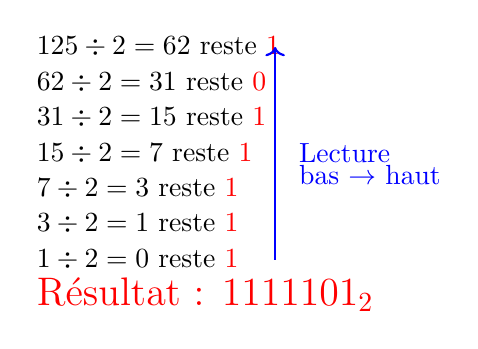
\begin{tikzpicture}[scale=0.9]
        \node[anchor=west] at (0,3.5) {$125 \div 2 = 62$ reste \textcolor{red}{1}};
        \node[anchor=west] at (0,3.0) {$62 \div 2 = 31$ reste \textcolor{red}{0}};
        \node[anchor=west] at (0,2.5) {$31 \div 2 = 15$ reste \textcolor{red}{1}};
        \node[anchor=west] at (0,2.0) {$15 \div 2 = 7$ reste \textcolor{red}{1}};
        \node[anchor=west] at (0,1.5) {$7 \div 2 = 3$ reste \textcolor{red}{1}};
        \node[anchor=west] at (0,1.0) {$3 \div 2 = 1$ reste \textcolor{red}{1}};
        \node[anchor=west] at (0,0.5) {$1 \div 2 = 0$ reste \textcolor{red}{1}};

        \draw[->,thick,blue] (3.5,0.5) -- (3.5,3.5);
        \node[anchor=west,blue] at (3.7,2) {Lecture};
        \node[anchor=west,blue] at (3.7,1.7) {bas $\rightarrow$ haut};

        \node[anchor=west,red,font=\Large] at (0,0) {Résultat : $1111101_2$};
      \end{tikzpicture}
    \end{column}
    \begin{column}{0.48\textwidth}
      \textbf{Binaire $\rightarrow$ Décimal}

      \textbf{Somme des puissances de 2}

      \small
      Exemple : $1111101_2 \rightarrow ?_{10}$

      \vspace{0.5em}

      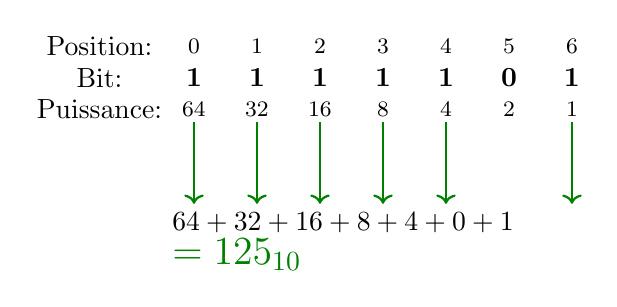
\begin{tikzpicture}[scale=0.8]
        \node at (0.5,3) {Position:};
        \node at (0.5,2.5) {Bit:};
        \node at (0.5,2) {Puissance:};

        \foreach \i/\b/\p in {1/1/64, 2/1/32, 3/1/16, 4/1/8, 5/1/4, 6/0/2, 7/1/1} {
          \node at (\i+1,3) {\footnotesize \the\numexpr\i-1};
          \node at (\i+1,2.5) {\textbf{\b}};
          \node at (\i+1,2) {\footnotesize \p};
          \ifnum\b=1
            \draw[->,thick,green!50!black] (\i+1,1.8) -- (\i+1,0.5);
          \fi
        }

        \node[anchor=west] at (1.5,0.2) {$64+32+16+8+4+0+1$};
        \node[anchor=west,green!50!black,font=\Large] at (1.5,-0.3) {$= 125_{10}$};
      \end{tikzpicture}
    \end{column}
  \end{columns}

\end{frame}

% %%%%%%%%%%%%%%%
% % SLIDE 11: Exercice conversion base 10 → autres bases
% %%%%%%%%%%%%%%%
\begin{frame}{Exercice : Convertir 125 en différentes bases}

  \textbf{Convertir le nombre 125 en :} a) Base 2, b) Base 8, c) Base 16

  \pause
  \textbf{a) Conversion en base 2 :} (cf slide précédent) $125_{10} = 1111101_2$

  \vspace{0.5em}

  \textbf{b) Conversion en base 8 :}
  \pause
  \begin{itemize}
    \item $125 \div 8 = 15$ reste 5
    \item $15 \div 8 = 1$ reste 7
    \item $1 \div 8 = 0$ reste 1
    \item Lecture de bas en haut : $175_8$
  \end{itemize}

  \textbf{c) Conversion en base 16 :}
  \pause
  \begin{itemize}
    \item $125 \div 16 = 7$ reste 13 (D)
    \item $7 \div 16 = 0$ reste 7
    \item Lecture de bas en haut : $7D_{16}$
  \end{itemize}

  \vspace{0.5em}

  \begin{exampleblock}{Vérification}
    On retrouve bien 125 depuis chaque base !
    \begin{itemize}
      \item $175_8 = 1 \cdot 64 + 7 \cdot 8 + 5 = 125$ 
      \item $7D_{16} = 7 \cdot 16 + 13 = 125$ 
    \end{itemize}
  \end{exampleblock}

\end{frame}

%%%%%%%%%%%%%%%
% SLIDE 12: Diagramme Binaire ↔ Hexa
%%%%%%%%%%%%%%%
\begin{frame}{Passerelle rapide Binaire $\leftrightarrow$ Hexadécimal}

  \begin{columns}
    \begin{column}{0.48\textwidth}
      \textbf{Binaire $\rightarrow$ Hexa}

      \textbf{Grouper par 4 bits (nibble)}

      \vspace{0.5em}

      Exemple : $11111101_2 = ?_{16}$

      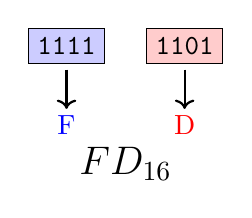
\begin{tikzpicture}
        \node[draw,fill=blue!20] at (0,1) {\texttt{1111}};
        \node[draw,fill=red!20] at (1.5,1) {\texttt{1101}};

        \draw[->,thick] (0,0.7) -- (0,0.2);
        \draw[->,thick] (1.5,0.7) -- (1.5,0.2);

        \node[blue] at (0,0) {F};
        \node[red] at (1.5,0) {D};

        \node[font=\Large] at (0.75,-0.5) {$FD_{16}$};
      \end{tikzpicture}
    \end{column}
    \begin{column}{0.48\textwidth}
      \textbf{Hexa $\rightarrow$ Binaire}

      \textbf{Développer chaque symbole en 4 bits}

      \vspace{0.5em}

      Exemple : $7D_{16} = ?_2$

      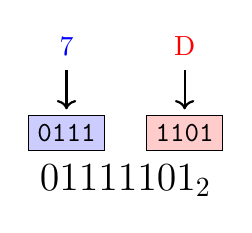
\begin{tikzpicture}
        \node[blue] at (0,1.5) {7};
        \node[red] at (1.5,1.5) {D};

        \draw[->,thick] (0,1.2) -- (0,0.7);
        \draw[->,thick] (1.5,1.2) -- (1.5,0.7);

        \node[draw,fill=blue!20] at (0,0.4) {\texttt{0111}};
        \node[draw,fill=red!20] at (1.5,0.4) {\texttt{1101}};

        \node[font=\Large] at (0.75,-0.2) {$01111101_2$};
      \end{tikzpicture}
    \end{column}
  \end{columns}


\end{frame}

%%%%%%%%%%%%%%%
% SLIDE 13: Représentation sur nombre de bits fixe
%%%%%%%%%%%%%%%
\begin{frame}[allowframebreaks]{Représentation sur un nombre de bits fixe}

  \textbf{Notation :} $^P(N_A)_B$

  Conversion de $N$ de la base $A$ vers la base $B$ sur \textbf{exactement} $P$ chiffres.

  \vspace{0.5em}

  \textbf{Exemples :}
  \begin{itemize}
    \item $^8(9_{10})_2 = 00001001_2$ (9 en binaire sur 8 bits)
    \item $^4(11_2)_{10} = 0003$ (11 binaire = 3, sur 4 chiffres)
  \end{itemize}

  \vspace{0.5em}

  \begin{block}{En programmation}
    Les entiers sont codés sur un nombre de bits fixe :

    \begin{center}
      \begin{tabular}{lcc}
        \hline
        \textbf{Type} & \textbf{Bits} & \textbf{Plage (non signé)} \\
        \hline
        \texttt{char / uint8\_t}  & 8 bits  & 0 à 255 \\
        \texttt{short / uint16\_t} & 16 bits & 0 à 65\,535 \\
        \texttt{int / uint32\_t}   & 32 bits & 0 à 4\,294\,967\,295 \\
        \texttt{long / uint64\_t}  & 64 bits & 0 à $2^{64}-1$ \\
        \hline
      \end{tabular}
    \end{center}
  \end{block}

  \vspace{0.5em}

  \pause
  \begin{alertblock}{Conséquence}
    $\rightarrow$ Risque de \textbf{débordement} !
  \end{alertblock}

\end{frame}

%%%%%%%%%%%%%%%
% SLIDE 14: Addition binaire
%%%%%%%%%%%%%%%
\begin{frame}[fragile]{Addition en binaire (nombres non signés)}
  \textbf{Principe :} Addition chiffre par chiffre, de droite à gauche, en propageant la retenue.
  Notation : $+_B$ pour l'addition dans la base $B$

  \vspace{0.5em}

  \textbf{Exemples :}
  \begin{columns}
    \begin{column}{0.3\textwidth}
      \textbf{En base 10 :}
      \begin{semiverbatim}
      81
    + 89
    ----
     170
      \end{semiverbatim}
    \end{column}
    \begin{column}{0.3\textwidth}
      \textbf{En base 16 :}
      \begin{semiverbatim}
      81
    + 89
    ----
     10A
      \end{semiverbatim}
    \end{column}
    \begin{column}{0.3\textwidth}
      \textbf{En base 2 :}
      \begin{semiverbatim}
     00101
   + 01110
   -------
     10011
      \end{semiverbatim}
      \small (5 + 14 = 19)
    \end{column}
  \end{columns}
\end{frame}

%%%%%%%%%%%%%%%
% SLIDE 15: Débordement
%%%%%%%%%%%%%%%
\begin{frame}[fragile]{Détection de débordement}

  Sur un format de $n$ bits : une retenue finale indique un \textbf{débordement} = résultat incorrect.

  \vspace{0.5em}

  \begin{columns}
    \begin{column}{0.48\textwidth}
      \textbf{SANS débordement : 28 + 5}

      \small
      \begin{semiverbatim}
  Retenue:     11
            00011100  (28)
          + 00000101  (5)
          ----------
            00100001  (33)
      \end{semiverbatim}

      Pas de retenue finale \\
      $\rightarrow$ \textcolor{green!50!black}{ Correct !}
    \end{column}
    \begin{column}{0.48\textwidth}
      \textbf{AVEC débordement : 128 + 129}

      \small
      \begin{semiverbatim}
  Retenue: 1
            10000000  (128)
          + 10000001  (129)
          ----------
          1 00000001  (1)
            ^
      \end{semiverbatim}

      \vspace{-2em}
      Retenue finale = 1 \\
      $\rightarrow$ \textcolor{red}{X DÉBORDEMENT}

      Résultat théorique : 257 \\
      Plage sur 8 bits : 0 à 255 \\
      $\rightarrow$ 257 non représentable
    \end{column}
  \end{columns}


  \pause
  \begin{alertblock}{Sur les processeurs}
    Un indicateur \textbf{C} (Carry) est positionné quand il y a débordement.

     En C, il faut gérer ces débordements soi-même !
  \end{alertblock}

\end{frame}

%%%%%%%%%%%%%%%
% SLIDE 16: Récapitulatif entiers non signés
%%%%%%%%%%%%%%%
\begin{frame}{Récapitulatif : Entiers non signés}

  \textbf{Ce qu'on a vu :}

  \begin{itemize}
    \item[\checkmark] \textbf{Conversion Base $B$ $\rightarrow$ Base 10 :} \\
          Somme des poids $\times$ puissances de $B$

    \item[\checkmark] \textbf{Conversion Base 10 $\rightarrow$ Base $B$ :} \\
          Divisions successives par $B$, lecture des restes

    \item[\checkmark] \textbf{Astuce Binaire $\leftrightarrow$ Hexa :} \\
          Groupement par nibbles (4 bits)

    \item[\checkmark] \textbf{Addition binaire :} \\
          Chiffre par chiffre avec propagation des retenues

    \item[\checkmark] \textbf{Débordement :} \\
          Retenue finale = indicateur C = overflow
  \end{itemize}

  \vspace{0.5em}

  \begin{block}{Limitations}
    \begin{itemize}
      \item Format fixe $\rightarrow$ plage limitée
      \item Pas de nombres négatifs pour l'instant
    \end{itemize}
    \textbf{Question :} Comment représenter $-5$ ?
  \end{block}

  \vspace{0.5em}


\end{frame}

%%%%%%%%%%%%%%%%%%%%%%%%%%%%%%%%%%%%%%%%%%%%%%%%%%%%%%%%%%%%
\section{Entiers signés}
%%%%%%%%%%%%%%%%%%%%%%%%%%%%%%%%%%%%%%%%%%%%%%%%%%%%%%%%%%%%


%%%%%%%%%%%%%%%
% SLIDE 17: Problème représentation signée
%%%%%%%%%%%%%%%
\begin{frame}[allowframebreaks, fragile]{Comment représenter des nombres négatifs ?}

  \textbf{Approche naïve : Bit de signe + Valeur absolue}

  \vspace{0.5em}

  Idée : Utiliser 1 bit pour le signe, le reste pour la valeur. \\
  Par exemple sur 4 bits : \texttt{[S][x$_2$][x$_1$][x$_0$]}
  \begin{itemize}
    \item S=0 $\rightarrow$ positif
    \item S=1 $\rightarrow$ négatif
  \end{itemize}

  Exemple : +3 = 0011$_2$, -3 = 1011$_2$

  \vspace{0.5em}

  \begin{alertblock}{Deux problèmes majeurs}
    \textbf{X Problème 1 : Double représentation du zéro}
    \begin{itemize}
      \item +0 = 0000$_2$
      \item -0 = 1000$_2$
      \item $\rightarrow$ Gaspillage d'un code
    \end{itemize}

    \textbf{X Problème 2 : L'addition ne fonctionne pas !}

    Calcul : (+3) + (-2) devrait donner +1
    \begin{semiverbatim}
     0011  (+3)
   + 1010  (-2)
   ------
     1101  → décodage = -5  xxx
    \end{semiverbatim}
  \end{alertblock}

\end{frame}

%%%%%%%%%%%%%%%
% SLIDE 18: Principe du code complément
%%%%%%%%%%%%%%%
\begin{frame}{Code complément : une meilleure approche}

  \textbf{Principe sur 4 bits (16 codes possibles) :}
  \begin{itemize}
    \item 8 codes pour les positifs : 0 à +7 $\rightarrow$ Codage classique : $^4(N)_2$
    \item 8 codes pour les négatifs : -8 à -1 $\rightarrow$ Codage spécial pour que l'addition fonctionne
  \end{itemize}

  \begin{block}{Équation fondamentale}
    \[
      ^P(N)_B +_B \, ^P(-N)_B = \, ^P(0)_B
    \]
    Le code du négatif doit être tel que son addition avec le positif donne 0 (en ignorant la retenue sortante).
  \end{block}

  \vspace{0.5em}

  \textbf{Exemple intuitif en base 10 sur 4 chiffres :}

  Pour trouver le code de -3 : \quad $0003 + ???? = 0000$ (en gardant 4 chiffres)

  Quelle valeur ajouter à 3 pour obtenir 0000 ?

  \[
    0003 + 9997 = 10000 \rightarrow \text{les 4 derniers chiffres} = 0000
  \]

  Donc : $^4(-3) = 9997$

  \vspace{0.3em}

  \textbf{Vérification :} $0003 + 9997 = 1|0000$ (on garde les 4 derniers) 

\end{frame}

%%%%%%%%%%%%%%%
% SLIDE 19: Notion de complément
%%%%%%%%%%%%%%%
\begin{frame}[allowframebreaks]{Définition mathématique du complément}

  \begin{block}{Complément d'un chiffre}
    Soit $x_B$ un chiffre en base $B$. \\
    Le complément de $x_B$, noté $x^*_B$, est défini par :
    \[
      x_B +_B x^*_B = (B-1)_B
    \]
  \end{block}

  \textbf{Exemples :}
  \begin{itemize}
    \item En base 2 : $1^*_2 = 0_2$ car $1_2 +_2 0_2 = 1_2$, \quad $0^*_2 = 1_2$ car $0_2 +_2 1_2 = 1_2$
    \item En base 8 : $1^*_8 = 6_8$ car $1_8 +_8 6_8 = 7_8$
    \item En base 16 : $1^*_{16} = E_{16}$ car $1_{16} +_{16} E_{16} = F_{16}$
  \end{itemize}

  \textbf{Propriété :} Le complément est involutif : $x^{**}_B = x_B$

  \vspace{0.5em}

  \begin{block}{Complément d'un nombre}
    Pour $^P(N)_B$ sur $P$ chiffres, on applique le complément à chaque chiffre.
  \end{block}

  \textbf{Exemples :}
  \begin{itemize}
    \item $01011000_2^* = 10100111_2$ (on inverse chaque bit)
    \item $108^* = 891$ (en base 10 sur 3 chiffres)
  \end{itemize}

\end{frame}

%%%%%%%%%%%%%%%
% SLIDE 20: Formule complément à 2
%%%%%%%%%%%%%%%
\begin{frame}{Complément à 2 : la formule}

  \begin{block}{Théorème}
    \[
      ^P(-N)_B = \, ^P(N)_B^* +_B 1
    \]
    C'est-à-dire : Code du négatif = Complément de chaque chiffre + 1
  \end{block}

  \vspace{0.5em}

  \textbf{Pourquoi ça marche ?}

  On sait que : $^P(N)_B +_B \, ^P(N)_B^* = B^P - 1$

  Donc : $B^P = (^P(N)_B +_B \, ^P(N)_B^*)_{10} + 1$

  Or on cherche : $^P(-N)_B = \, ^P(B^P - N)_B$

  En remplaçant : $^P(-N)_B = \, ^P((^P(N)_B^*)_{10} + 1)_B = \, ^P(N)_B^* +_B 1$ 


  \begin{exampleblock}{Méthode pratique pour coder un négatif}
    \begin{enumerate}
      \item Écrire le positif
      \item Inverser tous les chiffres
      \item Ajouter 1
    \end{enumerate}
  \end{exampleblock}

\end{frame}

%%%%%%%%%%%%%%%
% SLIDE 21: Exemple détaillé binaire
%%%%%%%%%%%%%%%
\begin{frame}[allowframebreaks, fragile]{Exemple : Coder -3 en base 2 sur 8 bits}

  \textbf{Étape 1 :} Coder +3 en binaire sur 8 bits
  \[
    ^8(3)_2 = 00000011_2
  \]

  \textbf{Étape 2 :} Inverser tous les bits (complément)
  \[
    00000011_2^* = 11111100_2
  \]

  \textbf{Étape 3 :} Ajouter 1
  \begin{semiverbatim}
      11111100
    +        1
    - - - - - - 
      11111101
  \end{semiverbatim}


  \begin{exampleblock}{Vérification}
    $00000011_2 + 11111101_2 = ?$
    \begin{semiverbatim}
  Retenue: 11111111 
            00000011  (+3)
          + 11111101  (-3)
          - - - - - - - - 
          1 00000000  (0) 
            ^
      On ignore la retenue sortante
    \end{semiverbatim}
    Le résultat est bien 0 !
  \end{exampleblock}

\end{frame}

%%%%%%%%%%%%%%%
% SLIDE 22: Exemple base 10
%%%%%%%%%%%%%%%
\begin{frame}[fragile]{Exemple : Coder -3 en base 10 sur 4 chiffres}

  \textbf{Étape 1 :} Coder +3 en base 10 sur 4 chiffres
  \[
    ^4(3) = 0003
  \]

  \textbf{Étape 2 :} Complémenter chaque chiffre (en base 10, le complément de $x$ est $9-x$)
  \[
    0003^* = 9996
  \]
  \begin{itemize}
    \item $0 \rightarrow 9$
    \item $3 \rightarrow 6$
  \end{itemize}

  \textbf{Étape 3 :} Ajouter 1
  \begin{semiverbatim}
      9996
    +    1
    - - - - - 
      9997
  \end{semiverbatim}



  On retrouve bien le résultat intuitif du slide 18 !

\end{frame}


%%%%%%%%%%%%%%%
% SLIDE 23: Exercice complément à 2
%%%%%%%%%%%%%%%
\begin{frame}{Exercice : Calculer des codes en complément à 2}

  \textbf{Questions :}

  \begin{enumerate}
    \item[a)] Code de 3 puis de -3 en base 2 sur 8 bits
    \item[b)] Code de 3 puis de -3 en base 4 sur 3 chiffres
    \item[c)] Code de -128 en base 2 sur 8 bits
    \item[d)] Code de -3 en base 16 sur 4 chiffres
  \end{enumerate}

  \vspace{1em}

  \textbf{Bonus :}
  \begin{itemize}
    \item[e)] Si $X = \,^P(-N)_B$, que vaut $X^* + 1$ ?
  \end{itemize}

\end{frame}

%%%%%%%%%%%%%%%
% SLIDE 24: Correction exercice
%%%%%%%%%%%%%%%
\begin{frame}{Correction}

  \textbf{a)} Base 2 sur 8 bits : $+3 = 00000011_2$, $-3 = 11111101_2$

  \textbf{b)} Base 4 sur 3 chiffres : $+3 = 003_4$
  \begin{itemize}
    \item Complément en base 4 : $0 \rightarrow 3$, $3 \rightarrow 0$
    \item $003_4^* = 330_4$
    \item $-3 = 330_4 + 1 = 331_4$
  \end{itemize}

  \textbf{c)} -128 en base 2 sur 8 bits :
  \begin{itemize}
    \item +128 ne tient pas sur 8 bits signés ! (max = 127)
    \item Mais -128 est représentable (min = -128)
    \item Astuce : $-128 = -2^7 = 10000000_2$
  \end{itemize}

  \textbf{d)} -3 en base 16 sur 4 chiffres :
  \begin{itemize}
    \item $+3 = 0003_{16}$, $0003_{16}^* = FFFC_{16}$, $-3 = FFFD_{16}$
  \end{itemize}

  \textbf{e)} Si $X = \,^P(-N)_B = \,^P(N)_B^* + 1$, alors :
  \[
    X^* + 1 = (^P(N)_B^* + 1)^* + 1 = \,^P(N)_B^{**} + \ldots = \,^P(N)_B
  \]
  $\rightarrow$ Le complément à 2 est involutif : $-(-N) = N$ 

\end{frame}

%%%%%%%%%%%%%%%
% SLIDE 25: Bit de signe
%%%%%%%%%%%%%%%
\begin{frame}[allowframebreaks]{Comment reconnaître un nombre négatif ?}

  \begin{block}{Propriété du code complément à 2}
    Le bit (ou chiffre) de poids fort indique le signe. En base 2 sur $n$ bits :
    \begin{itemize}
      \item Bit de poids fort = 0 $\rightarrow$ nombre positif ou nul
      \item Bit de poids fort = 1 $\rightarrow$ nombre négatif
    \end{itemize}

    On l'appelle le ``bit de signe''.
  \end{block}

  \textbf{Exemples sur 8 bits :}
  \begin{center}
    \begin{tabular}{lcc}
      \hline
      \textbf{Code} & \textbf{Bit signe} & \textbf{Valeur} \\
      \hline
      \textcolor{green}{0} 0000000 & 0 & +0 \\
      \textcolor{green}{0} 0000011 & 0 & +3 \\
      \textcolor{green}{0} 1111111 & 0 & +127 (max) \\
      \textcolor{red}{1} 0000000 & 1 & -128 (min) \\
      \textcolor{red}{1} 1111101 & 1 & -3 \\
      \textcolor{red}{1} 1111111 & 1 & -1 \\
      \hline
    \end{tabular}
  \end{center}

  \begin{block}{Plage sur $n$ bits}
    \[
      \left[ -2^{n-1} , 2^{n-1} - 1 \right]
    \]
    Sur 8 bits : $[-128, +127]$ (256 valeurs, asymétrique)
  \end{block}

  \begin{alertblock}{Différence avec signe + valeur absolue}
    Le bit de poids fort n'est PAS simplement collé devant la valeur !
  \end{alertblock}

\end{frame}

% ============================================================================
% Slide 26 : Exercice Complément à 2 (Décodage)
% ============================================================================
\begin{frame}{Exercice : Décodage en Complément à 2}

  \begin{exampleblock}{Consigne}
    Convertissez les nombres binaires suivants (codés sur 8 bits en complément à 2) en décimal :
  \end{exampleblock}

  \vspace{0.3cm}

  \begin{enumerate}
    \item $A = 0101\ 1010_2$
    \item $B = 1000\ 0001_2$
    \item $C = 1111\ 1111_2$
    \item $D = 0111\ 1111_2$
  \end{enumerate}

  \vspace{0.3cm}
  \pause

  \begin{alertblock}{Méthode}
    \begin{itemize}
      \item Si bit de poids fort = 0 → nombre positif → conversion classique
      \item Si bit de poids fort = 1 → nombre négatif → formule du complément à 2
    \end{itemize}
  \end{alertblock}

\end{frame}

% ============================================================================
% Slide 27 : Correction de l'exercice
% ============================================================================
\begin{frame}{Correction : Décodage en Complément à 2}

  \begin{itemize}
    \item \textbf{a)} $A = 0101\ 1010_2$ → Bit de poids fort = \textcolor{green}{0} → positif

    \[
      A = 64 + 16 + 8 + 2 = \textbf{90}_{10}
    \]

    \pause
    \item \textbf{b)} $B = 1000\ 0001_2$ → Bit de poids fort = \textcolor{red}{1} → négatif

    \[
      B = -128 + 1 = \textbf{-127}_{10}
    \]

    \pause
    \item \textbf{c)} $C = 1111\ 1111_2$ → Bit de poids fort = \textcolor{red}{1} → négatif

    \[
      C = -128 + 64 + 32 + 16 + 8 + 4 + 2 + 1 = -128 + 127 = \textbf{-1}_{10}
    \]

    \pause
    \item \textbf{d)} $D = 0111\ 1111_2$ → Bit de poids fort = \textcolor{green}{0} → positif

    \[
      D = 64 + 32 + 16 + 8 + 4 + 2 + 1 = \textbf{127}_{10}
    \]
    (Valeur maximale sur 8 bits signés !)
  \end{itemize}

\end{frame}

% ============================================================================
% Slide 28 : Addition de nombres signés
% ============================================================================
\begin{frame}{Addition de nombres signés}

  \begin{block}{Principe}
    L'addition fonctionne \textbf{exactement pareil} qu'avec des nombres non signés !
    On additionne bit par bit avec retenues, puis on ignore la retenue finale.
  \end{block}

  \vspace{0.3cm}

  \textbf{Exemple 1 : $5 + (-3) = 2$} sur 8 bits.

  \begin{center}
    \begin{tabular}{r|ccccccccc}
      Retenue & \textcolor{blue}{1} & 1 & 1 & 1 & 1 & 1 &  & 1 & \\
      \hline
      $+5$ &  & 0 & 0 & 0 & 0 & 0 & 1 & 0 & 1 \\
      $-3$ & & 1 & 1 & 1 & 1 & 1 & 1 & 0 & 1 \\
      \hline
      Résultat & \textcolor{blue}{1} & 0 & 0 & 0 & 0 & 0 & 0 & 1 & 0 \\
    \end{tabular}
  \end{center}

  \vspace{0.2cm}

  On ignore la retenue finale (en bleu) → $0000\ 0010_2 = +2$


  \begin{alertblock}{Remarque importante}
    Le matériel n'a besoin que d'un seul additionneur pour signés ET non signés !
  \end{alertblock}

\end{frame}

% ============================================================================
% Slide 29 : Détection du débordement (overflow)
% ============================================================================
\begin{frame}{Débordement (overflow)}

  \begin{block}{Problème}
    Que se passe-t-il si le résultat d'une opération dépasse la plage $[-128, +127]$ ?
  \end{block}

  \vspace{0.3cm}

  \textbf{Exemple : $100 + 50 = 150$ (overflow !)}

  \begin{center}
    \begin{tabular}{r|cccccccc}
      Retenue & 0 & 1 & 1 & 1 & 0 & 0 & 0 & 0 \\
      \hline
      $+100$ & 0 & 1 & 1 & 0 & 0 & 1 & 0 & 0 \\
      $+50$ & 0 & 0 & 1 & 1 & 0 & 0 & 1 & 0 \\
      \hline
      Résultat & \textcolor{red}{1} & 0 & 0 & 1 & 0 & 1 & 1 & 0 \\
    \end{tabular}
  \end{center}

  \vspace{0.2cm}

  Résultat : $1001\ 0110_2 = -106$ en complément à 2 (absurde !)


  \begin{alertblock}{Détection du débordement signé (flag V ou OV)}
    \textbf{Overflow} si et seulement si $\text{retenue entrante dans bit de poids fort} \neq \text{retenue sortante}$. Ici : entrante = 0, sortante = 1 → V = 1 (overflow détecté !)
  \end{alertblock}

\end{frame}

% % ============================================================================
% % Slide 30 : Roue des nombres signés
% % ============================================================================
\begin{frame}{Visualisation : La roue des nombres signés}

  \begin{columns}
    \begin{column}{0.5\textwidth}
      \begin{center}
        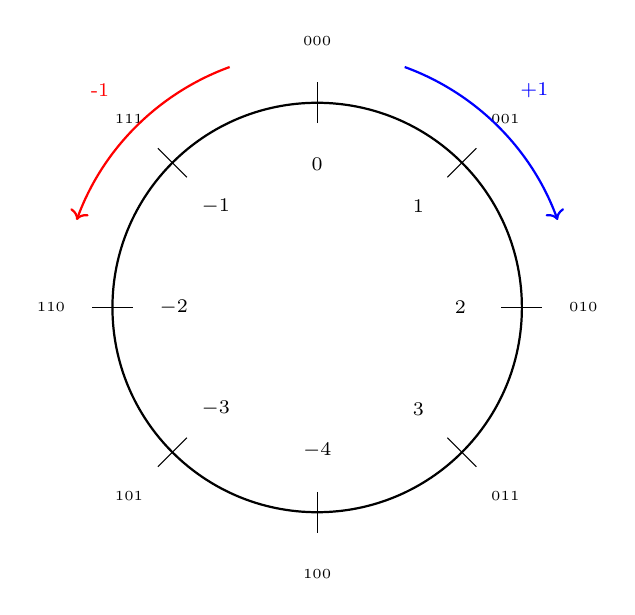
\begin{tikzpicture}[scale=1.3]
          % Cercle
          \draw[thick] (0,0) circle (2cm);

          % Divisions
          \foreach \angle/\val/\bin in {
            90/0/000,
            45/1/001,
            0/2/010,
            -45/3/011,
            -90/-4/100,
            -135/-3/101,
            -180/-2/110,
            -225/-1/111
          } {
            \draw (\angle:1.8cm) -- (\angle:2.2cm);
            \node at (\angle:1.4cm) {\scriptsize $\val$};
            \node at (\angle:2.6cm) {\tiny $\bin$};
          }

          % Flèche sens horaire
          \draw[->,thick,blue] (70:2.5cm) arc (70:20:2.5cm);
          \node[blue] at (45:3cm) {\scriptsize +1};

          % Flèche sens anti-horaire
          \draw[->,thick,red] (110:2.5cm) arc (110:160:2.5cm);
          \node[red] at (135:3cm) {\scriptsize -1};

        \end{tikzpicture}
      \end{center}
    \end{column}

    \begin{column}{0.5\textwidth}
      \begin{block}{Sur 3 bits}
        Plage : $[-4, +3]$
      \end{block}

      \vspace{0.5cm}

      \textbf{Exemples :}
      \begin{itemize}
        \item $3 + 1 = 100_2 = -4$ (overflow)
        \item $-4 - 1 = 011_2 = +3$ (overflow)
        \item $-1 + 1 = 000_2 = 0$ 
      \end{itemize}

      \vspace{0.5cm}

      \begin{alertblock}{Propriété}
        Le complément à 2 forme une \textbf{arithmétique modulaire} : les nombres "bouclent" !
      \end{alertblock}
    \end{column}
  \end{columns}

\end{frame}
%
% % ============================================================================
% % Slide 31 : Récapitulatif Entiers signés
% % ============================================================================
\begin{frame}{ Récapitulatif : Entiers signés}

  \begin{block}{Complément à 2 (standard universel)}
    \begin{itemize}
      \item Plage sur $n$ bits : $\left[ -2^{n-1}, 2^{n-1}-1 \right]$
      \item Bit de poids fort = bit de signe (0 → positif, 1 → négatif)
      \item Formule de décodage : $^P(-N)_2 = -b_{n-1} \cdot 2^{n-1} + \sum_{i=0}^{n-2} b_i \cdot 2^i$
      \item Encodage de $-X$ : inverser tous les bits de $X$ puis ajouter 1
    \end{itemize}
  \end{block}

  \begin{alertblock}{Avantages}
     Un seul zéro (contrairement à signe + valeur absolue) \\
     Addition/soustraction identiques aux non signés \\
     Matériel simplifié
  \end{alertblock}

  \begin{exampleblock}{Détection de débordement}
    \begin{itemize}
      \item \textbf{Non signés} : flag C (carry) = retenue sortante
      \item \textbf{Signés} : flag V/OV (overflow) = retenue entrante $\neq$ retenue sortante
    \end{itemize}
  \end{exampleblock}

\end{frame}
%
% % ============================================================================
% % SECTION 4 : Nombres flottants
% % ============================================================================
\section{Nombres à virgule flottante}
%
% ============================================================================
% Slide 32 : Introduction aux nombres flottants
% ============================================================================
\begin{frame}{Nombres à virgule flottante}

  \begin{block}{Problème avec les entiers}
    Les entiers ne peuvent représenter que des nombres entiers ! \\
    Comment coder $3.14159$, $0.0001$, $6.022 \times 10^{23}$ ?
  \end{block}

  \vspace{0.3cm}

  \textbf{Deux approches :}

  \begin{enumerate}
    \item \textbf{Virgule fixe} : nombre fixe de bits pour la partie entière et fractionnaire
    \begin{itemize}
      \item Exemple : 8 bits entiers + 8 bits fractionnaires
      \item Limité en plage et en précision
    \end{itemize}

    \pause

    \item \textbf{Virgule flottante} (standard IEEE 754) : notation scientifique en binaire
    \begin{itemize}
      \item Signe + Mantisse + Exposant
      \item Très grande plage dynamique
      \item \textbf{Standard universel} sur tous les ordinateurs modernes
    \end{itemize}
  \end{enumerate}


  \begin{alertblock}{Attention}
    Les flottants ont des \textbf{limitations de précision} !
  \end{alertblock}

\end{frame}

% ============================================================================
% Slide 33 : Virgule fixe (aperçu rapide)
% ============================================================================
\begin{frame}{Virgule fixe (Fixed-Point)}

  \begin{block}{Principe}
    On réserve un nombre fixe de bits pour la partie entière et la partie fractionnaire.
  \end{block}

  \vspace{0.3cm}

  \textbf{Exemple sur 16 bits : 8.8 (8 bits entiers, 8 bits fractionnaires)}

  \begin{center}
    \begin{tabular}{|c|c|}
      \hline
      \textbf{Partie entière (8 bits)} & \textbf{Partie fractionnaire (8 bits)} \\
      \hline
      $2^7 \ldots 2^1\ 2^0$ & $2^{-1}\ 2^{-2} \ldots 2^{-7}\ 2^{-8}$ \\
      \hline
    \end{tabular}
  \end{center}

  \vspace{0.3cm}

  \textbf{Exemple : $5.75_{10}$}

  \begin{itemize}
    \pause
    \item Partie entière : $5 = 0000\ 0101_2$
    \pause
    \item Partie fractionnaire : $0.75 = 0.5 + 0.25 = 2^{-1} + 2^{-2} = 1100\ 0000_2$
    \pause
    \item Résultat : $0000\ 0101\ .\ 1100\ 0000$
  \end{itemize}


  \begin{alertblock}{Limites}
     Plage restreinte (sur 8.8 : de 0 à 255.996) \\
     Pas de nombres très grands ou très petits ($10^{23}$ ou $10^{-10}$)
  \end{alertblock}

\end{frame}

% ============================================================================
% Slide 34 : IEEE 754 - Vue d'ensemble
% ============================================================================
\begin{frame}{IEEE 754 : Norme universelle}

  \begin{block}{Principe}
    Représentation en \textbf{notation scientifique binaire} :
    \[
      \text{Nombre} = (-1)^S \times (1.M) \times 2^{E - \text{biais}}
    \]
  \end{block}

  \vspace{0.3cm}

  \textbf{Format simple précision (32 bits) :}

  \begin{center}
    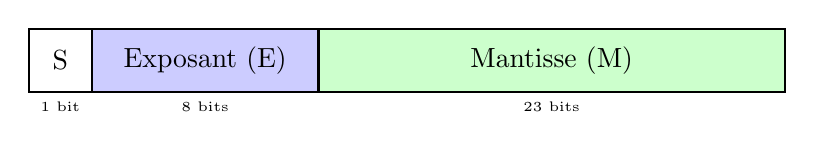
\begin{tikzpicture}[scale=0.8]
      % Signe
      \draw[thick] (0,0) rectangle (1,1);
      \node at (0.5,0.5) {S};
      \node[below] at (0.5,0) {\tiny 1 bit};

      % Exposant
      \draw[thick,fill=blue!20] (1,0) rectangle (4.6,1);
      \node at (2.8,0.5) {Exposant (E)};
      \node[below] at (2.8,0) {\tiny 8 bits};

      % Mantisse
      \draw[thick,fill=green!20] (4.6,0) rectangle (12,1);
      \node at (8.3,0.5) {Mantisse (M)};
      \node[below] at (8.3,0) {\tiny 23 bits};
    \end{tikzpicture}
  \end{center}


  \begin{itemize}
    \item \textbf{S} (1 bit) : signe (0 = positif, 1 = négatif)
    \item \textbf{E} (8 bits) : exposant biaisé (biais = 127)
    \item \textbf{M} (23 bits) : mantisse (partie fractionnaire, bit implicite = 1)
  \end{itemize}



\end{frame}
%
% ============================================================================
% Slide 35 : Exemple de décodage IEEE 754
% ============================================================================
\begin{frame}{Exemple : Décodage IEEE 754}

  \textbf{Soit le nombre codé sur 32 bits :}

  \begin{center}
    \texttt{0 10000010 01000000000000000000000}
  \end{center}

  \vspace{0.3cm}

  \textbf{Décomposition :}

  \begin{itemize}
    \item \textbf{S} = 0 → nombre positif
    \item \textbf{E} = $10000010_2 = 130_{10}$
    \item \textbf{M} = $01000000000000000000000_2 = 0.25_{10}$ (en binaire : $0.01_2 = 2^{-2}$)
  \end{itemize}

  \vspace{0.3cm}

  \textbf{Calcul :}
  
  \vspace{-2em}
  \begin{align*}
    \text{Valeur} &= (-1)^0 \times (1 + 0.25) \times 2^{(130 - 127)} \\
                  &= 1 \times 1.25 \times 2^3 \\
                  &= 1.25 \times 8 \\
                  &= \textbf{10.0}
  \end{align*}

\end{frame}

% ============================================================================
% Slide 36 : Exercice interactif - Décodage IEEE 754
% ============================================================================
\begin{frame}{Exercice : Décodage IEEE 754}

  \begin{exampleblock}{Consigne}
    Décodez le nombre IEEE 754 suivant (32 bits) :

    \begin{center}
      \texttt{1 01111100 10000000000000000000000}
    \end{center}
  \end{exampleblock}

  \vspace{0.5cm}

  \textbf{Étapes :}

  \begin{enumerate}
    \item Extraire S, E, M
    \item Convertir E en décimal
    \item Convertir M en décimal
    \item Appliquer la formule : $(-1)^S \times (1.M) \times 2^{(E-127)}$
  \end{enumerate}



\end{frame}

% ============================================================================
% Slide 37 : Correction de l'exercice
% ============================================================================
\begin{frame}{Correction : Décodage IEEE 754}

  \texttt{1 01111100 10000000000000000000000}

  \vspace{0.3cm}

  \textbf{Décomposition :}

  \begin{itemize}
    \item \textbf{S} = 1 → nombre \textcolor{red}{négatif}
    \item \textbf{E} = $01111100_2 = 124_{10}$
    \item \textbf{M} = $10000000000000000000000_2 = 0.5_{10}$ \\
          (en binaire : $0.1_2 = 2^{-1} = 0.5$)
  \end{itemize}

  \vspace{0.3cm}

  \textbf{Calcul :}

  \begin{align*}
    \text{Valeur} &= (-1)^1 \times (1 + 0.5) \times 2^{(124 - 127)} \\
                  &= -1 \times 1.5 \times 2^{-3} \\
                  &= -1.5 \times \frac{1}{8} \\
                  &= -1.5 \times 0.125 \\
                  &= \textbf{-0.1875}
  \end{align*}

\end{frame}

% ============================================================================
% Slide 38 : Codage d'un nombre en IEEE 754
% ============================================================================
\begin{frame}{Codage d'un nombre en IEEE 754}

  \textbf{Étapes pour coder un nombre (ex : $-6.5$) :}

  \vspace{0.3cm}

  \begin{enumerate}
    \item \textbf{Signe} : $-6.5$ est négatif → S = 1

    \pause

    \item \textbf{Conversion en binaire} : $6.5 = 110.1_2$ \\
          (car $6 = 110_2$ et $0.5 = 0.1_2$)

    \pause

    \item \textbf{Normalisation} : écrire sous forme $1.M \times 2^{\text{exp}}$ \\
          $110.1_2 = 1.101_2 \times 2^2$

    \pause

    \item \textbf{Exposant biaisé} : $E = 2 + 127 = 129 = 10000001_2$

    \pause

    \item \textbf{Mantisse} : M = partie après "1." → $101$ complété à 23 bits : \\
          $10100000000000000000000$
  \end{enumerate}

  \vspace{0.3cm}

  \textbf{Résultat final :}

  \begin{center}
    \texttt{1 10000001 10100000000000000000000}
  \end{center}

\end{frame}

% ============================================================================
% Slide 39 : Valeurs spéciales IEEE 754
% ============================================================================
\begin{frame}{Valeurs spéciales IEEE 754}

  \begin{center}
    \begin{tabular}{|l|l|l|l|}
      \hline
      \textbf{Valeur} & \textbf{S} & \textbf{E (8 bits)} & \textbf{M (23 bits)} \\
      \hline
      \hline
      $+0$ & 0 & $00000000$ & $00000000000000000000000$ \\
      \hline
      $-0$ & 1 & $00000000$ & $00000000000000000000000$ \\
      \hline
      \hline
      $+\infty$ & 0 & $11111111$ & $00000000000000000000000$ \\
      \hline
      $-\infty$ & 1 & $11111111$ & $00000000000000000000000$ \\
      \hline
      \hline
      NaN (Not a Number) & X & $11111111$ & $\neq 0$ (quelconque) \\
      \hline
    \end{tabular}
  \end{center}

  \vspace{0.5cm}

  \begin{exampleblock}{Exemples d'opérations produisant NaN}
    \begin{itemize}
      \item $\frac{0}{0}$, $\infty - \infty$, $\sqrt{-1}$
      \item NaN se propage : toute opération avec NaN donne NaN
    \end{itemize}
  \end{exampleblock}


  \begin{alertblock}{ Attention}
    IEEE 754 distingue $+0$ et $-0$ (mais sont égaux en comparaison)
  \end{alertblock}

\end{frame}

% ============================================================================
% Slide 40 : Pièges des flottants
% ============================================================================
\begin{frame}[fragile]{ Pièges des nombres flottants}

  \begin{alertblock}{Piège 1 : Précision limitée (arrondi)}
    De nombreux nombres décimaux n'ont PAS de représentation binaire exacte !
  \end{alertblock}

  \vspace{0.3cm}

  \textbf{Exemple classique : $0.1 + 0.2 \neq 0.3$ en flottant !}

  \begin{lstlisting}[language=Python,basicstyle=\small\ttfamily]
>>> 0.1 + 0.2
0.30000000000000004
  \end{lstlisting}

  \vspace{0.3cm}

  \textbf{Raison :} $0.1_{10} = 0.0001100110011\ldots_2$ (période infinie en binaire !)

  \vspace{0.5cm}

  \begin{exampleblock}{Règle d'or}
    \textbf{Ne JAMAIS comparer deux flottants avec ==} \\
    À la place : $|a - b| < \varepsilon$ (avec $\varepsilon$ très petit, ex : $10^{-9}$)
  \end{exampleblock}

\end{frame}



% ============================================================================
% SECTION 5 : Caractères
% ============================================================================
\section{Représentation des caractères}

% ============================================================================
% Slide 43 : Histoire des encodages
% ============================================================================
\begin{frame}{Représentation des caractères}

  \begin{block}{Problème}
    Comment représenter les lettres, chiffres, symboles sous forme binaire ?
  \end{block}

  \vspace{0.3cm}

  \textbf{Historique des encodages :}

  \begin{enumerate}
    \item \textbf{ASCII (1963)} : 7 bits, 128 caractères (alphabet anglais)
    \begin{itemize}
      \item A-Z, a-z, 0-9, ponctuation, caractères de contrôle
    \end{itemize}

    \pause

    \item \textbf{Variantes nationales (années 70-80)} : ISO-8859-1 (Latin-1), etc.
    \begin{itemize}
      \item 8 bits, 256 caractères (ajout des accents européens)
      \item  Incompatibilités entre pays !
    \end{itemize}

    \pause

    \item \textbf{Unicode (1991)} : norme universelle pour TOUS les caractères
    \begin{itemize}
      \item Plus de 149 000 caractères (toutes les langues, émojis, etc.)
      \item Encodages : UTF-8, UTF-16, UTF-32
    \end{itemize}
  \end{enumerate}

\end{frame}

% ============================================================================
% Slide 44 : Table ASCII
% ============================================================================
\begin{frame}{Table ASCII (7 bits, 128 caractères)}

  \begin{center}
    \small
    \begin{tabular}{|c|c|c|c||c|c|c|c|}
      \hline
      \textbf{Dec} & \textbf{Hex} & \textbf{Bin} & \textbf{Char} & \textbf{Dec} & \textbf{Hex} & \textbf{Bin} & \textbf{Char} \\
      \hline
      32 & 20 & 0100000 & (espace) & 65 & 41 & 1000001 & A \\
      33 & 21 & 0100001 & ! & 66 & 42 & 1000010 & B \\
      \ldots & \ldots & \ldots & \ldots & \ldots & \ldots & \ldots & \ldots \\
      48 & 30 & 0110000 & 0 & 90 & 5A & 1011010 & Z \\
      49 & 31 & 0110001 & 1 & 97 & 61 & 1100001 & a \\
      \ldots & \ldots & \ldots & \ldots & 98 & 62 & 1100010 & b \\
      57 & 39 & 0111001 & 9 & \ldots & \ldots & \ldots & \ldots \\
      \hline
    \end{tabular}
  \end{center}

  \vspace{0.3cm}

  \begin{exampleblock}{Points clés}
    \begin{itemize}
      \item \textbf{A-Z} : codes 65 à 90 (majuscules)
      \item \textbf{a-z} : codes 97 à 122 (minuscules, décalage de +32)
      \item \textbf{0-9} : codes 48 à 57 (chiffres)
      \item Codes 0-31 : caractères de contrôle (retour chariot, tabulation, etc.)
    \end{itemize}
  \end{exampleblock}

\end{frame}

% ============================================================================
% Slide 45 : Exercice ASCII
% ============================================================================
\begin{frame}{Exercice : Décodage ASCII}

  \begin{exampleblock}{Consigne}
    Décodez la séquence hexadécimale suivante en texte ASCII :

    \begin{center}
      \texttt{49 4E 46 4F 35 30 31}
    \end{center}
  \end{exampleblock}


  \textbf{Méthode :} Convertir chaque octet en décimal, puis chercher dans la table ASCII.


  \pause

  \begin{block}{Correction}
    \small
    \begin{itemize}
      \setlength\itemsep{0em}
      \item $49_{16} = 73_{10}$ → 'I'
      \item $4E_{16} = 78_{10}$ → 'N'
      \item $46_{16} = 70_{10}$ → 'F'
      \item $4F_{16} = 79_{10}$ → 'O'
      \item $35_{16} = 53_{10}$ → '5'
      \item $30_{16} = 48_{10}$ → '0'
      \item $31_{16} = 49_{10}$ → '1'
    \end{itemize}

  \end{block}

\end{frame}

% ============================================================================
% Slide 46 : Limites de l'ASCII
% ============================================================================
\begin{frame}{Limites de l'ASCII}

  \begin{alertblock}{ Problèmes de l'ASCII}
    \begin{itemize}
      \item \textbf{Limité à 128 caractères} (7 bits) → pas d'accents !
      \item Extensions nationales (ISO-8859-1, Windows-1252, etc.) \textbf{incompatibles} entre elles
      \item Impossible de représenter les langues non-latines (chinois, arabe, cyrillique, etc.)
      \item Pas d'émojis, symboles mathématiques avancés, etc.
    \end{itemize}
  \end{alertblock}

  \vspace{0.3cm}

  \textbf{Exemple de problème :}

  \begin{itemize}
    \item Un fichier avec des "é" codé en Latin-1 lu en UTF-8 → "é"
    \item Un email en cyrillique lu avec l'encodage japonais → illisible !
  \end{itemize}


  \begin{block}{Solution : Unicode}
    Norme universelle assignant un \textbf{point de code} unique à chaque caractère de toutes les langues du monde !
  \end{block}

\end{frame}

% ============================================================================
% Slide 47 : Unicode et UTF-8
% ============================================================================
\begin{frame}[allowframebreaks]{Unicode et UTF-8}

  \begin{block}{Unicode}
    \begin{itemize}
      \item Norme définissant plus de 149 000 caractères
      \item Chaque caractère a un \textbf{point de code} noté U+XXXX (en hexa)
      \item Exemples : U+0041 = 'A', U+00E9 = 'é', U+1F600 = :) (à imaginer)
    \end{itemize}
  \end{block}


  \begin{block}{UTF-8 : encodage dominant (web, Linux, etc.)}
    \textbf{Encodage à longueur variable} : 1 à 4 octets par caractère

    \begin{itemize}
      \item \textbf{1 octet} : caractères ASCII (0-127) → compatibilité totale !
      \item \textbf{2 octets} : accents, cyrillique, arabe, hébreu, etc.
      \item \textbf{3 octets} : chinois, japonais, coréen
      \item \textbf{4 octets} : émojis, caractères rares
    \end{itemize}
  \end{block}

  \framebreak
  \begin{exampleblock}{Avantage de UTF-8}
     Rétrocompatible avec ASCII \\
     Économise de l'espace pour les textes latins \\
     Standard du web (>98\% des sites)
  \end{exampleblock}

\begin{table}
\captionsetup{labelformat=empty}
\caption{Code point $\leftrightarrow$ UTF-8 conversion}
\begin{tabular}{|l|l|l|l|l|l|}
\hline First code point & Last code point & Byte 1 & Byte 2 & Byte 3 & Byte 4 \\
\hline U+0000 & U+007F & 0yyyzzzz & & & \\
\hline U+0080 & U+07FF & 110xxxyy & 10yyzzzz & & \\
\hline U+0800 & U+FFFF & 1110wwww & 10xxxxyy & 10yyzzzz & \\
\hline U+010000 & U+10FFFF & 11110uvv & 10vvwwww & 10xxxxyy & 10yyzzzz \\
\hline
\end{tabular}
\end{table}

\end{frame}

% ============================================================================
% Slide 48 : Exemple UTF-8
% ============================================================================
\begin{frame}{Exemple : Encodage UTF-8}

  \textbf{Caractère : 'é' (e accent aigu)}

  \begin{itemize}
    \item \textbf{Point de code Unicode :} U+00E9 (décimal : 233)
    \item \textbf{Encodage UTF-8 :} 2 octets : \texttt{C3 A9}
  \end{itemize}

  \vspace{0.3cm}

  \textbf{Décomposition :}

  \begin{center}
    \begin{tabular}{|c|c|}
      \hline
      \textbf{Octet 1} & \textbf{Octet 2} \\
      \hline
      \texttt{11000011} (C3) & \texttt{10101001} (A9) \\
      \hline
    \end{tabular}
  \end{center}

  \vspace{0.3cm}

  \begin{itemize}
    \item Premier octet commence par \texttt{110} → caractère sur 2 octets
    \item Deuxième octet commence par \texttt{10} → octet de continuation
    \item Bits de données : \texttt{00011 101001} = $233_{10}$ 
  \end{itemize}

  \vspace{0.5cm}

  \textbf{Émoji : :) (U+1F600)}

  \begin{itemize}
    \item \textbf{Encodage UTF-8 :} 4 octets : \texttt{F0 9F 98 80}
  \end{itemize}

\end{frame}
%
% % ============================================================================
% % Slide 49 : Art ASCII
% % ============================================================================
\begin{frame}[fragile]{Art ASCII (pour le plaisir !)}

  \begin{lstlisting}[basicstyle=\tiny\ttfamily]
 ________      ___   __       ______     ______       ______      ______       ____        
/_______/\    /__/\ /__/\    /_____/\   /_____/\     /_____/\    /_____/\     /___/\       
\__.::._\/    \::\_\\  \ \   \::::_\/_  \:::_ \ \    \::::_\/_   \:::_ \ \    \_::\ \      
   \::\ \      \:. `-\  \ \   \:\/___/\  \:\ \ \ \    \:\/___/\   \:\ \ \ \     \::\ \     
   _\::\ \__    \:. _    \ \   \:::._\/   \:\ \ \ \    \_::._\:\   \:\ \ \ \    _\: \ \__  
  /__\::\__/\    \. \`-\  \ \   \:\ \      \:\_\ \ \    /_____\/    \:\_\ \ \  /__\: \__/\ 
  \________\/     \__\/ \__\/    \_\/       \_____\/    \_____/      \_____\/  \________\/ 
  \end{lstlisting}

  \vspace{0.3cm}

  \begin{center}
    Chaque caractère est codé en ASCII ! \\
    Art créé uniquement avec des caractères imprimables.
  \end{center}

  \vspace{0.5cm}

  \begin{exampleblock}{Anecdote}
    L'art ASCII était populaire dans les années 80-90 avant l'arrivée des interfaces graphiques.
    On le retrouve encore dans les \texttt{README}, bannières de logiciels CLI, etc.
  \end{exampleblock}

\end{frame}

% ============================================================================
% Slide 50 : Récapitulatif Caractères
% ============================================================================
\begin{frame}[allowframebreaks]{ Récapitulatif : Caractères}

  \begin{block}{ASCII (1963)}
    \begin{itemize}
      \item 7 bits, 128 caractères (alphabet anglais + contrôle)
      \item A = 65, a = 97, 0 = 48
      \item Base de tous les encodages modernes
    \end{itemize}
  \end{block}

  \begin{block}{Unicode (1991)}
    \begin{itemize}
      \item Norme universelle : >149 000 caractères (toutes langues + émojis)
      \item Point de code : U+XXXX (notation hexadécimale)
    \end{itemize}
  \end{block}

  \framebreak

  \begin{block}{UTF-8 (encodage dominant)}
    \begin{itemize}
      \item Longueur variable : 1 à 4 octets
      \item Rétrocompatible avec ASCII (1 octet pour 0-127)
      \item Standard du web (>98\%)
    \end{itemize}
  \end{block}

  \begin{alertblock}{ Attention}
    Toujours spécifier l'encodage lors de la lecture/écriture de fichiers texte !
  \end{alertblock}

\end{frame}

% ============================================================================
% SECTION 6 : Exercices finaux
% ============================================================================
\section{Exercices de synthèse}

% ============================================================================
% Slide 51 : Exercice 1 - Transstockeur
% ============================================================================
\begin{frame}{Exercice 1 : Transstockeur (version simplifiée)}

  \begin{exampleblock}{Contexte}
    Un transstockeur industriel utilise des adresses codées sur 12 bits :
    \begin{itemize}
      \item 4 bits pour l'allée (A)
      \item 4 bits pour la travée (T)
      \item 4 bits pour le niveau (N)
    \end{itemize}
    Format : \texttt{AAAA TTTT NNNN}
  \end{exampleblock}

  \vspace{0.3cm}

  \textbf{Questions :}

  \begin{enumerate}
    \item Combien d'emplacements différents peut-on adresser ?
    \item Quelle est l'adresse (en binaire et en hexa) de l'emplacement : \\
          Allée 5, Travée 12, Niveau 3 ?
    \item Décodez l'adresse hexadécimale \texttt{0x7A9}.
  \end{enumerate}


\end{frame}

% ============================================================================
% Slide 52 : Correction Exercice 1
% ============================================================================
\begin{frame}{Correction : Transstockeur}

  \textbf{1) Nombre d'emplacements :}

  \[
    2^{12} = 4096 \text{ emplacements}
  \]

  (ou $2^4 \times 2^4 \times 2^4 = 16 \times 16 \times 16 = 4096$)

  \vspace{0.3cm}

  \textbf{2) Encodage de (Allée 5, Travée 12, Niveau 3) :}

  \begin{itemize}
    \item Allée 5 : $5 = 0101_2$
    \item Travée 12 : $12 = 1100_2$
    \item Niveau 3 : $3 = 0011_2$
  \end{itemize}

  Adresse binaire : $0101\ 1100\ 0011_2$ \\
  Adresse hexa : $0x5C3$

  \vspace{0.3cm}

  \textbf{3) Décodage de 0x7A9 :}

  $0x7A9 = 0111\ 1010\ 1001_2$

  \begin{itemize}
    \item Allée : $0111_2 = 7$
    \item Travée : $1010_2 = 10$
    \item Niveau : $1001_2 = 9$
  \end{itemize}

  \textbf{Résultat :} Allée 7, Travée 10, Niveau 9

\end{frame}

% ============================================================================
% Slide 53 : Exercice 2 - Numération mixte
% ============================================================================
\begin{frame}{Exercice 2 : Numération et arithmétique}

  \textbf{a) Conversions :}

  \begin{enumerate}
    \item Convertir $237_{10}$ en binaire, octal, et hexadécimal
    \item Convertir $10110011_2$ en décimal et hexadécimal
  \end{enumerate}

  \vspace{0.3cm}

  \textbf{b) Addition binaire sur 8 bits (non signés) :}

  Calculer $01101101_2 + 00111010_2$. Y a-t-il débordement (carry) ?

  \vspace{0.3cm}

  \textbf{c) Complément à 2 sur 8 bits :}

  \begin{enumerate}
    \item Encoder $-42$ en complément à 2
    \item Décoder $11010110_2$ (complément à 2)
  \end{enumerate}



\end{frame}

% ============================================================================
% Slide 54 : Correction Exercice 2
% ============================================================================
\begin{frame}{Correction : Numération et arithmétique}

  \textbf{a) Conversions de $237_{10}$ :}

  \begin{itemize}
    \item Binaire : $237 = 128 + 64 + 32 + 8 + 4 + 1 = 11101101_2$
    \item Octal : $237 \div 8 = 29$ reste 5, $29 \div 8 = 3$ reste 5, $3 \div 8 = 0$ reste 3 → $355_8$
    \item Hexa : $11101101_2 = 1110\ 1101 = \text{ED}_{16}$
  \end{itemize}

  \textbf{Conversions de $10110011_2$ :}

  \begin{itemize}
    \item Décimal : $128 + 32 + 16 + 2 + 1 = 179_{10}$
    \item Hexa : $1011\ 0011 = \text{B3}_{16}$
  \end{itemize}

  \vspace{0.3cm}

  \textbf{b) Addition :} $01101101_2 + 00111010_2$

  \[
    01101101 + 00111010 = 10100111_2 \quad \text{(pas de retenue sortante)} \rightarrow \text{Carry} = 0
  \]

  Résultat : $10100111_2 = 167_{10}$ (pas de débordement)

\end{frame}

% ============================================================================
% Slide 55 : Correction Exercice 2 (suite)
% ============================================================================
\begin{frame}{Correction : Complément à 2}

  \textbf{c.1) Encoder $-42$ en complément à 2 (8 bits) :}

  \begin{enumerate}
    \item Encoder $+42$ : $42 = 00101010_2$
    \item Inverser tous les bits : $11010101_2$
    \item Ajouter 1 : $11010101 + 1 = 11010110_2$
  \end{enumerate}

  \textbf{Résultat :} $-42 = 11010110_2$

  \vspace{0.5cm}

  \textbf{c.2) Décoder $11010110_2$ (complément à 2) :}

  Bit de poids fort = 1 → négatif

  \[
    -128 + 64 + 16 + 4 + 2 = -128 + 86 = \textbf{-42}_{10}
  \]

   Cohérent avec l'encodage précédent !

\end{frame}

% ============================================================================
% Slide 56 : Exercice 3 - Flottant IEEE 754
% ============================================================================
\begin{frame}{Exercice 3 : IEEE 754 (optionnel / avancé)}

  \begin{exampleblock}{Question}
    Encoder le nombre $-12.5$ en IEEE 754 simple précision (32 bits).
  \end{exampleblock}

  \vspace{0.3cm}

  \textbf{Étapes suggérées :}

  \begin{enumerate}
    \item Déterminer le signe (S)
    \item Convertir $12.5$ en binaire
    \item Normaliser sous forme $1.M \times 2^{\text{exp}}$
    \item Calculer l'exposant biaisé (E)
    \item Extraire la mantisse (M) sur 23 bits
    \item Assembler : S | E (8 bits) | M (23 bits)
  \end{enumerate}

  \vspace{0.3cm}

  \pause

  \begin{alertblock}{Indice}
    $12.5_{10} = 12 + 0.5 = 1100_2 + 0.1_2 = 1100.1_2$
  \end{alertblock}

\end{frame}

% ============================================================================
% Slide 57 : Correction Exercice 3
% ============================================================================
\begin{frame}{Correction : IEEE 754 ($-12.5$)}

  \textbf{1) Signe :} $-12.5$ est négatif → S = 1

  \vspace{0.2cm}

  \textbf{2) Conversion binaire :} $12.5 = 1100.1_2$ \\
  (car $12 = 1100_2$ et $0.5 = 0.1_2$)

  \vspace{0.2cm}

  \textbf{3) Normalisation :} $1100.1_2 = 1.1001_2 \times 2^3$

  \vspace{0.2cm}

  \textbf{4) Exposant biaisé :} $E = 3 + 127 = 130 = 10000010_2$

  \vspace{0.2cm}

  \textbf{5) Mantisse :} M = partie après "1." → $1001$ complété à 23 bits : \\
  $10010000000000000000000$

  \vspace{0.3cm}

  \textbf{Résultat final :}

  \begin{center}
    \fbox{\texttt{1 10000010 10010000000000000000000}}
  \end{center}

  En hexadécimal : \texttt{0xC1480000}

\end{frame}

% ============================================================================
% Slide 58 : Conclusion
% ============================================================================
\begin{frame}{Conclusion}

  \begin{block}{Ce que nous avons vu aujourd'hui}
    \begin{itemize}
      \item \textbf{Notion de codage} : tout est binaire en machine
      \item \textbf{Entiers non signés} : conversions, bases 2/8/16, arithmétique
      \item \textbf{Entiers signés} : complément à 2, débordement
      \item \textbf{Nombres flottants} : IEEE 754, pièges, bugs célèbres
      \item \textbf{Caractères} : ASCII, Unicode, UTF-8
    \end{itemize}
  \end{block}


  \begin{alertblock}{ Points clés à retenir}
    \begin{itemize}
      \item Les nombres ont une \textbf{plage limitée} (overflow possibles)
      \item Les flottants ont une \textbf{précision limitée} (ne jamais comparer avec ==)
      \item Les caractères dépendent de l'\textbf{encodage} (toujours spécifier UTF-8 !)
    \end{itemize}
  \end{alertblock}



\end{frame}

% ============================================================================
% Slide 59 : BONUS - Démo en direct
% ============================================================================
\begin{frame}{BONUS }

  \begin{center}
    {\Huge \textbf{Manipulation de la mémoire en hexadécimal}}
  \end{center}

  \vspace{1cm}

  \begin{block}{Ce que nous allons voir}
    \begin{itemize}
      \item Lancer un mini-jeu qui affiche ses variables en mémoire
      \item Affichage en temps réel : hexadécimal
      \item Modifier la mémoire avec un débogueur
      \item Observer le changement instantané des valeurs
    \end{itemize}
  \end{block}


  \begin{center}
    {\Large \textbf{Passons à la démo...}}
  \end{center}

\end{frame}

% ============================================================================
% Fin du document
% ============================================================================
\end{document}
